\lecture{22}{2024-11-28}{Orhogonalité}{}

Soit $A$ une matrice diagonalisable. Il existe une matrice inversible $P$ et une matrice diagonale $D$ telles que:
\[A = PDP^{-1}\]
Mais alors on a aussi 
\[A^2 = PDP^{-1}PDP^{-1} = PD^2P^{-1} \text{ et } A^k = PD^kP^{-1}\]


\[
D =
\begin{pmatrix}
\lambda_1 & 0 & \cdots & 0 \\
0 & \lambda_2 & \cdots & 0 \\
\vdots & \vdots & \ddots & \vdots \\
0 & 0 & \cdots & \lambda_n
\end{pmatrix}
\quad \Rightarrow \quad
D^k =
\begin{pmatrix}
\lambda_1^k & 0 & \cdots & 0 \\
0 & \lambda_2^k & \cdots & 0 \\
\vdots & \vdots & \ddots & \vdots \\
0 & 0 & \cdots & \lambda_n^k
\end{pmatrix}
\]

\begin{parag}{Evolution de populations}
    On étudie les populations de Lausanne et du Gros de Vaud. La situation (sans lien avec la réalité du canton) est représenté par la situation suivante:
    \begin{center}
        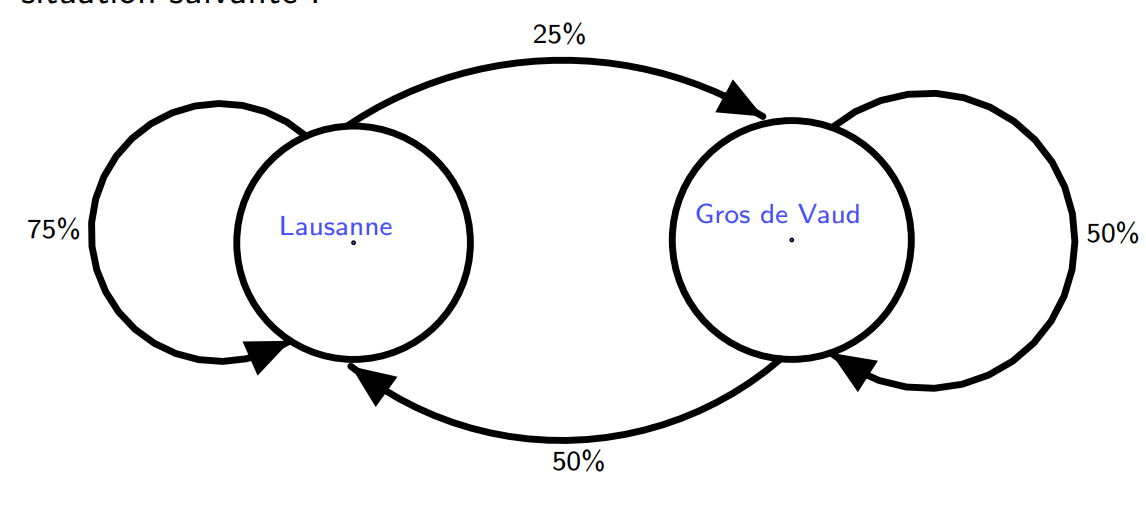
\includegraphics[scale=0.4]{Algèbre linéàaire/Screenshot 2024-11-28 081103.png}
    \end{center}
    Appelons $u_k$ la population urbaine l'année $k$ (en pourcents) et $r_k$ la population rurale.
    \\ 
    On cherche ici à écrire une formule pour décrire tout ça.\\
    \[u_{k+1} = \frac{3}{4}u_k + \frac{1}{2}r_k\]
    
    \[r_{k+1} = \frac{1}{4}u_k + \frac{1}{2}r_k\]
    On a donc:
    \[\begin{cases}
        u_{k+1} = \frac{3}{4}u_k + \frac{1}{2}r_k\\
        r_{k+1} = \frac{1}{4}u_k + \frac{1}{2}r_k
    \end{cases}\]
    Nous avons modélisé matriciellemment cette situtation et posons:
\[A = \begin{pmatrix}
    3/4 & 1/2\\ 1/4 & 1/2
\end{pmatrix}\]
Ainsi:
\[\begin{pmatrix}
    3/4 & 1/2\\ 1/4 & 1/2
\end{pmatrix}\begin{pmatrix}
    u_k \\ r_k
\end{pmatrix} = \begin{pmatrix}
    u_{k+1}\\ r_{k+1}
\end{pmatrix}\]
si bien que:
\[\begin{pmatrix}
    3/4 & 1/2\\ 1/4 & 1/2
\end{pmatrix}^k\begin{pmatrix}
    u_0\\r_0
\end{pmatrix} = \begin{pmatrix}
    u_k \\ r_k
\end{pmatrix}\]
Pour comprendre ce qui se passe dans le futur (lointain), il faut donc calculer $\lim_{k \to \infty} A^k$.
\\
\\
Nous calculons:
\begin{enumerate}
    \item $c_A(t) = (t-1)(t-\frac{1}{4})$
    \item $E_1 = Vect\left\{\begin{pmatrix}
        2 \\ 1
    \end{pmatrix}\right\}$ et $E_{1/4} = Vect\left\{\begin{pmatrix}
        1 \\ -1
    \end{pmatrix}\right\}$
    \item $\bmath = \left(\begin{pmatrix}
        2\\1
    \end{pmatrix}, \begin{pmatrix}
        1 \\ -1
    \end{pmatrix}\right)$ est une base de \R$^2$ formée de vecteurs propres de $A$
    \item $P = (Id)_\bmath^{\cmath an} = \begin{pmatrix}
        2 & 1 \\ 1 & -1
    \end{pmatrix},\; P^{-1} = (Id)_{\cmath an}^\bmath = \frac{1}{3}\begin{pmatrix}
        1 & 1 \\ 1 & -2
    \end{pmatrix}$
    \item On a donc pour la diagonale: $D = \begin{pmatrix}
        1 & 0 \\ 0 & 1/4
    \end{pmatrix}$
    \item \textcolor{red}{Formule de changement de base } : $A^k = PD^kP^{-1}$.
\end{enumerate}
On va donc chercher maintenant à partir de la diagonale avec notre formuel énconcé au point $5$:
\[A^k = \frac{1}{3}\begin{pmatrix}
    2 & 1 \\ 1 & -1
\end{pmatrix}\begin{pmatrix}
    1^k & 0 \\ 0 & \frac{1}{4}^k
\end{pmatrix}\begin{pmatrix}
    1 & 1 \\ 1 & -2
\end{pmatrix} \\
= \frac{1}3{\begin{pmatrix}
    2+\frac{1}{4}^k & 2 -\frac{1}{4}^{k-1}\\
    1 - \frac{1}{4}^k & 1 + \frac{1}{4}^{k-1}
\end{pmatrix}}\]

\begin{align*}
    \begin{pmatrix}
        u_k\\r_k
    \end{pmatrix} = A^k\begin{pmatrix}
        u_0\\r_0
    \end{pmatrix} = \begin{pmatrix}
        1/3(2+\frac{1}{4}^k)u_0 + \frac{1}{3}(2-\frac{1}{4}^{k-1})r_0\\
        1/3(1-\frac{1}{4}^k)u_0 + \frac{1}{3}(1 + \frac{1}{4}^{k-1})r_0
    \end{pmatrix}
\end{align*}
Comme $\lim_{k\to \infty} \frac{1}{4}^k = 0$ on peut facilement trouver que $u_\infty = \frac{1}{3}\cdot2 u_0 = \frac{2}{3}P_0$ où $P_0 = u_0 + r_0$ qui est la population totale
\end{parag}


\chapter{Orthogonalité}
\begin{parag}{non}
    

\begin{enumerate}
    \item \R$^n$ est non seulement un espace vectoriel, c'est un espace \textcolor{red}{euclidien}.
    \item  Nous avons une notion de distance et d'angle
    \item La base canonique est composée de vecteurs \textcolor{red}{orthgonaux} deux à deux et \textcolor{red}{unitaires} (de longueur 1).
\end{enumerate}

\end{parag}

\begin{parag}{Le produit scalaire}
    \begin{definition}
        Soit $\vec{u}, \vec{v}$ deux vecteur de $\mathbb{R}^n$. Le \textcolor{red}{produit scalaire} est
        \begin{formule}
            \[\vec{u}\cdot\vec{v}= \vec{u}^t\vec{v} = u_1v_1 + \cdots + u_nv_n\]
        \end{formule}
    \end{definition}
    \begin{subparag}{Propriétés}
\begin{enumerate}
    \item \textbf{Commutativité} 
    $\vec{u} \cdot \vec{v} = \vec{v} \cdot \vec{u}$
    
    \item \textbf{Distributivité} 
    $\vec{u} \cdot (\vec{v} + \vec{w}) = \vec{u} \cdot \vec{v} + \vec{u} \cdot \vec{w}$
    
    \item \textbf{Compatibilité avec l'action scalaire}
    $\alpha (\vec{u} \cdot \vec{v}) = \vec{u} \cdot (\alpha \vec{v}) = (\alpha \vec{u}) \cdot \vec{v}$
    
    \item \textbf{Positivité} 
    $\vec{u} \cdot \vec{u} \geq 0 \quad \text{et} \quad \vec{u} \cdot \vec{u} = 0 \iff \vec{u} = \vec{0}$
\end{enumerate}

    \end{subparag}
    \begin{subparag}{Preuve}
        Les propriétés $1-3$ sont celles de la multiplication de matrice. Pour $4$, $\vec{u}\cdot\vec{u} = u_1^2 + \cdots + u_n^2\geq 0.$ On a l'égalité si et seulement si tous les $u_1 = 0$.
    \end{subparag}
\end{parag}
\begin{parag}{La norme}
    \begin{definition}
        La \textcolor{red}{longueur} ou \textcolor{red}{norme} d'une vecteur $\vec{u}$ de $\mathbb{R}^n$ est :
        \begin{formule}
            \[||\vec{u}|| = \sqrt{\vec{u}\cdot\vec{u}} = \sqrt{u_1^2 + \cdots + u_n^2}\]
        \end{formule}
    \end{definition}
    Un vecteur de norme $1$ est dit \textcolor{red}{unitaire}. Pour normaliser un vecteur non nul, il suffit de le diviser par sa norme:
    \[
\frac{\vec{u}}{\|\vec{u}\|} =
\begin{pmatrix}
\frac{u_1}{\|\vec{u}\|} \\
\vdots \\
\frac{u_n}{\|\vec{u}\|}
\end{pmatrix}
\quad \text{est unitaire}
\]


\end{parag}
\begin{parag}{La distance}
    \begin{definition}
        La \textcolor{red}{distance} entre deux vecteurs $\vec{u}$ et $\vec{v}$ de \R$^n$ est:
        \begin{formule}
            \[d(\vec{u}, \vec{v}) = ||\vec{u} - \vec{v}||\]
        \end{formule}
    \end{definition}
    \begin{framedremark}
        On voit aussi que cette formule marche dans l'autre sens.\\
        Des vecteurs sont orthogonaux si et seulement si la distance entre $\vec{u}$ et $\vec{v}$ est la même que la distance entre $\vec{u}$ et $-\vec{v}$.
    \end{framedremark}
    \begin{subparag}{Remarque}
        Quelles sont les conséquences de l'égalité $d(\vec
        {u}, \vec{v}) = d(\vec{u}, -\vec{v})$?\\
        Si $||\vec{u} - \vec{v}|| = ||\vec{u} - (-\vec{v})|| = || \vec{u}+\vec{v}||$ alors, $||\vec{u}-\vec{v}||^2 = ||\vec{u} + \vec{v}||^2$ on a le droit de dire ça car une distante est toujours positive.
        \\
        Par la définition de la norme:
        $(\vec{u} - \vec{v})\cdot(\vec{u}-\vec{v}) = (\vec{u}+\vec{v})\cdot(\vec{u}+\vec{v})$.
        \\
        Par la distributivité:
        \[\]
    \end{subparag}
    \begin{definition}
        Deux vecteurs $\vec{u}$ et $\vec{v}$ de $\mathbb{R}^n$ sont \textcolor{red}{orthogonaux} si 
        \begin{formule}
            \[\vec{u}\cdot \vec{v} = 0\]
        \end{formule}
    \end{definition}
        \begin{subparag}{Théorème de pythagore}
            \begin{theoreme}
                Deux vecteurs $\vec{u}$ et $\vec{v}$ sont orthogonaux si et seulement si 
                \[||\vec{u}+\vec{v}||^2 = ||\vec{u}||^2 + ||\vec{v}||^2\]
            \end{theoreme}
        \end{subparag}
        \begin{subparag}{Notation}
            Soit $W$ un sous-espace de $\mathbb{R}^n$. On note $W^\perp$ l'ensemble de tous les vecteurs orthofobaux à $W$. Ainsi;
            \begin{formule}
                \[W^\perp = \{\vec{u} \in \mathbb{R}^n| \vec{u} \cdot \vec{v} = 0 \text{ pour tout } \vec{w} \in W\}\]
            \end{formule}
            C'est un sous-espace de $\mathbb{R}^n$ (série 11)
        \end{subparag}
        \begin{subparag}{Exemple}
            Soit $W$ le sousespace de $\mathbb{R}^3$ donné par 'éaquation $2x -y + 3z = 0$. On veut décrire ce plan et $W^\perp$.
            \\
            On choisit une base de $W$ : 
            \[\bmath = \left(\begin{pmatrix}
                1 \\ 2 \\ 0
            \end{pmatrix}, \begin{pmatrix}
                -3 \\ 0 \\ 2
            \end{pmatrix}\right)\]
            On a donc par sa définition:
            \begin{align*}
              W^\perp &= \{\vec{u} \in \mathbb{R}^3|  \vec
            u\cdot \vec{w} = 0 \;\;\;\forall \vec{w} \in W\}\\  
            &= \{\vec{u} \in \mathbb{R}^3|\vec{u}\cdot(\alpha\vec{b_1} + \beta\vec{b_2}) = 0 \; \forall\alpha, \beta \in \mathbb{R}\}\\
            &= \{\vec{u} \in \mathbb{R}^3| \vec{u}\cdot\vec{b_1} = 0 = \vec{u}\cdot\vec{b_2}\}
            \end{align*}

            
            Si $\vec{u} = \begin{pmatrix}
                a \\ b \\ c
            \end{pmatrix}$ on a alors: 
            $\vec{u} \cdot \vec{b}_1 = a + 2b$ et $\vec{u}\cdot \vec{b_2} = -3a + 2c$
            On cherche donc à résoudre : 
            \[\begin{cases}
                a + 2b = 0\\
                -3a + 2c = 0
            \end{cases}\; \; , W^\perp = Vect\left\{\begin{pmatrix}
                2 \\ -1 \\ 3
            \end{pmatrix}\right\}\]
            \\
            On observe que $\begin{pmatrix}
                2 \\ -1 \\ 3 
            \end{pmatrix}\perp$ le plan d'éq. $2x -y + 3z = 0$
        \end{subparag}

\end{parag}

\begin{parag}{Lien entre perpendicularité et image et noyau}
    \begin{subparag}{Proposition}
        La droite perpendiculaire au plan déquation $ac + by + cz = 0$, et passant par l'origine \R$^3$, est engendrée par $\begin{pmatrix}
            a \\b \\ c
        \end{pmatrix}$.
    \end{subparag}
    \begin{theoreme}
        Soit $A$ une matrice de taille $m \times n$
        \begin{enumerate}
            \item $\ker A = (LignA)^\perp$
            \item $(ImA)^\perp = \ker(A^T)$
        \end{enumerate}
    \end{theoreme}
    \begin{subparag}{Preuve}
        \begin{enumerate}
            \item $A\cdot\vec{c} = \vec{0} \Leftrightarrow \vec{x}\perp$ chaque ligne de $A$.
            \item  $ImA = ColA = Lign(A^T)$ et $[Lign(A^T)]^\perp = \ker(A^T)$
        \end{enumerate}
    \end{subparag}

\end{parag}

\begin{parag}{Calcul d'angle}
 Le produit scalaire permet aussi de calculer l'angle entre deux vecteurs:
 \begin{theoreme}
     Loi du cosinus:
     \[\vec{u}\cdot \vec{v} = ||\vec{u}||\cdot ||\vec{v}||\cos \alpha\]
 \end{theoreme}
 Le produit scalaire de deux vecteurs est:
 \begin{enumerate}
     \item Nul quand $\cos\alpha = 0$ les vecteurs sont perpendiculaire
     \item maximal quand $\cos \alpha = 1$ les vecteurs sont colinéaire et de même sens
     \item minimmal quand $\cos\alpha = -1$.Les vecteurs sont colinéaires et de sens opposé.
 \end{enumerate}
\end{parag}

\begin{parag}{Famille orthogonales}
    \begin{definition}
        Une famille $\{\vec{u_1}, \dots, \vec{u_k}\}$ des vecteurs de $\mathbb{R}^n$ est \textcolor{red}{orthogonale} si $\vec{u_i}\perp \vec{u_j}$ pour tout $i \neq j$. Cette famille est \textcolor{red}{orthonormée} si de plus $||\vec{u_i}|| = 1$ pour tout $i$.
    \end{definition}
    \begin{subparag}{Exemple}
        La base canonique $(\vec{e_1}, \dots, \vec{e_n})$ est orthonormée. En général on appelle Base orthogonale de $W$ une famille orthogonale orfdonnée qui forme une base de $W$. de même pour une base orthonormée.
    \end{subparag}
    \begin{theoreme}
        Une famille orthogonale de vecteurs non nuls est libres.
    \end{theoreme}
    \begin{subparag}{Preuve}
        Soit une famille orthogonale de $\mathbb{R}^n$ avec $\vec{u_i \neq 0 \; \forall 1 \leq i \leq k}$. Soit $\alpha_1, \dots, \alpha_k \in \mathbb{R}$ et supposons $\alpha_1 \vec{u_1} + \cdots + \alpha_k\vec{u_k} = \vec{0}$. \\
        On doit montrer que $\alpha_1 = \cdots = \alpha_k = 0$.
        \\
        On calcule $0 = (\alpha_1\vec{u_1} + \cdots + \alpha_k\vec{u_k})\cdot \vec{u_i}$\\
        Par la ditributivité on a que c'est égal à $ = \alpha_1\vec{u_1}\cdot\vec{u_i} + \cdots + \alpha_k\vec{u_k}\cdot\vec{u_i}$\\
        Mais comme $\vec{u_i}\perp\vec{u_j}$ alors la seule possibilité est que tout les $\alpha_i = 0$
        
        
    \end{subparag}
\end{parag}


\begin{parag}{Coordonnées dans une base orthogonale}
    \begin{theoreme}
        Pour tout vecteur $\vec{w} \in W$, on a $\vec{w} = \alpha_1\vec{u_1} + \cdots + \alpha_k\vec{u_k}$ et 
        \begin{formule}
            \[\alpha_j = \frac{\vec{w}\cdot\vec{u_j}}{||\vec{u_j}||^2}\]
        \end{formule}
    \end{theoreme}
    On voit ici que la preuve sera du même principe que d'autre déjà faite 
    \begin{subparag}{Exemple}
    On construit une base orthogonale de $\mathbb{R}^3$ en commençant avec le plan d'équation $2x - 3y + z = 0$
    On choisit une base:
    \[\bmath = \left(\begin{pmatrix}
        3 \\ 2 \\ 0
    \end{pmatrix}, \begin{pmatrix}
        -2 \\ 3 \\ 13
    \end{pmatrix}\right) \; \text{ qui est une base orthogonale de W}\]
    \[\cmath = \left(\begin{pmatrix}
        3 \\ 2 \\ 0
    \end{pmatrix}, \begin{pmatrix}
        -2 \\ 3 \\ 13
    \end{pmatrix}\right)\]
    \end{subparag}
\end{parag}